\documentclass[11pt]{article}

\usepackage[margin=1in]{geometry}
\usepackage{amsmath, amssymb, amsthm}
\usepackage{microtype}
\usepackage{graphicx}
\usepackage[hidelinks]{hyperref}

\newtheorem{theorem}{Theorem}
\newtheorem{corollary}{Corollary}
\newtheorem{lemma}{Lemma}
\theoremstyle{remark}
\newtheorem*{remark}{Remark}

\newcommand{\Mhash}{\mathsf{M}}
\newcommand{\SHA}{\mathrm{SHA\text{-}256}}
\newcommand{\SHAd}{\mathrm{SHA\text{-}256d}}
\newcommand{\MAJ}{\mathrm{MAJ}}
\newcommand{\Ch}{\mathrm{Ch}}
\newcommand{\Maj}{\mathrm{Maj}}
\newcommand{\bigO}{\mathcal{O}}

% =====================================================================
% TITLE + ABSTRACT: authored last, after the body is settled.
% =====================================================================
\title{\textbf{The Carry Adder Wall}}
\author{Peter Hollows}
\date{\today}

\begin{document}
\maketitle

\begin{abstract}
Bitcoin mining searches for a block header whose double-SHA-256 hash
falls below a target, a weak-preimage problem solved in practice by
brute force. We ask whether any classical algorithm beats brute force,
and answer it by decomposing SHA-256d into two layers with opposite
properties. The message schedule is a fixed recurrence whose computation
is shareable across candidates. We show that every sharing
win is confined to three known, bounded regions (midstate caching, the
ASICBoost message-expansion region, and a provably unshareable second
hash), so the per-candidate cost is close to fixed. The round function
is pseudorandom. We prove, in the random-oracle model, that the
expected candidate count cannot fall below $2^{D}$, a
bound that survives preprocessing (Bitcoin is salted) and quantum search
(Grover gives only a quadratic speedup), and we reduce the
standard-model claim to a SHA-256 distinguisher. We then explain why the
round function resists prediction: the carry chain of modular addition is
its only position-coupling nonlinearity. We introduce \emph{carry depth},
the count of carry layers between a controllable input and a target
output, as a coordinate of the proof-of-work function space; we compute
it exactly at $386$ layers for SHA-256d, and we measure that the
strongest local advantage we tested falls below detection (consistent
with zero) within a single round. That single-round collapse, not the
size of the in-round advantage, is the empirical content; the strongest
local attack we tested therefore expires roughly $100$ rounds before
reaching the output. We are explicit about the ceiling: the result is
conditional on the carry/local attack class, and the entire residual
reduces to a global algebraic shortcut that would constitute a SHA-256
break, whose unconditional exclusion is, in the asymptotic framing, the
$\mathsf{P}\ne\mathsf{NP}$ problem.
\end{abstract}

% =====================================================================
\section{The mining search problem}
% =====================================================================

Bitcoin mining is a search problem over an iterated hash. A block header
$H$ is $80$ bytes; the mining hash is the double application
\[
  \Mhash(H) \;=\; \SHA\!\big(\SHA(H)\big),
\]
read as a $256$-bit integer. Mining succeeds when a miner finds an $H$
(within its allowed degrees of freedom: the $32$-bit nonce, the
coinbase extranonce that varies the Merkle root, version bits, and the
timestamp) such that $\Mhash(H) < T$, where $T = 2^{256}\cdot 2^{-D}$
and $D$ is the difficulty expressed in leading zero bits. Equivalently,
$H$ must land in a target set $S \subseteq \{0,1\}^{256}$ of density
$|S|/2^{256} = 2^{-D}$.

The question is operational: \emph{is there any classical algorithm that
finds such an $H$ at materially less expected cost than brute force?}
Brute force tries candidates until one lands in $S$, at expected cost
$\approx 2^{D}$ evaluations. An attack ``beats'' it only if it reduces the
total work by more than a constant factor.

\paragraph{Cost model.}
The atomic unit is one $\SHA$ compression-function call
$h:\{0,1\}^{256}\times\{0,1\}^{512}\to\{0,1\}^{256}$. It applies the
block cipher $E$ (SHACAL-2, keyed by the message $m$) to the chaining
value and feeds the input forward by \emph{wordwise modular addition},
$h(C,m) = C \boxplus E_m(C)$, where $\boxplus$ adds each of the eight
$32$-bit words modulo $2^{32}$. The feed-forward is thus itself a carry
operation, which matters in Section~\ref{sec:carry}. One header
evaluation decomposes into exactly three compression calls,
\[
\underbrace{C_1 = h(\mathrm{IV},B_0)}_{\text{block 0 (nonce-independent)}},\quad
\underbrace{C_2 = h(C_1,B_1\Vert\mathrm{pad})}_{\text{block 1 (nonce in word }W_3)},\quad
\underbrace{\mathrm{out}=h(\mathrm{IV},C_2\Vert\mathrm{pad})}_{\text{second hash}},
\]
with $B_0$ the first $64$ header bytes and $B_1$ the remaining $16$ plus
padding. Total mining cost is the number of candidate evaluations
multiplied by the compression calls per candidate that sharing cannot
remove. These two factors are governed by different structure, which the
next section makes precise.

% =====================================================================
\section{Two layers}\label{sec:twolayers}
% =====================================================================

The analysis rests on one structural fact: $\SHAd$ is built from two
kinds of structure with opposite properties.

\begin{center}
\begin{tabular}{ll p{0.36\textwidth}}
\hline
\textbf{layer} & \textbf{property} & \textbf{consequence}\\
\hline
message schedule & fixed recurrence (same per block) & computation is \emph{shareable} across candidates\\
round / compression & pseudorandom & output is \emph{unpredictable}; search is \emph{irreducible}\\
\hline
\end{tabular}
\end{center}

The only avenues to beat brute force live in one layer or the other:
either reduce the \emph{per-candidate cost} by sharing schedule
computation (Section~\ref{sec:amort}), or reduce the \emph{candidate
count} by predicting or skipping evaluations
(Sections~\ref{sec:search}--\ref{sec:carry}). We show the first avenue is
bounded to known constant-factor techniques, and the second is
impossible in the ideal model and equivalent to breaking $\SHA$ in the
standard model. Because the two avenues act on different layers, a gain
in one neither requires nor enables a gain in the other, and the rest of
the paper addresses them in turn.

% =====================================================================
\section{The amortization envelope}\label{sec:amort}
% =====================================================================

Written as a product, the cost is
\[
  \text{cost} \;\ge\;
  \underbrace{(\text{candidate evaluations})}_{\text{locked at }2^D,\ \S\ref{sec:search}}
  \;\times\;
  \underbrace{(\text{compressions per candidate after maximal sharing})}_{\text{this section}}.
\]
The left factor is locked at $2^{D}$ by the search lower bound. Hence any
economically meaningful win against brute force must come from the right
factor: per-candidate computation sharing. We bound it by classifying
which of the three compressions can be shared across \emph{distinct}
candidates.

\begin{itemize}
\item \textbf{Block~0 (midstate).} Nonce-independent, and shared across
  the entire nonce sweep of a fixed header prefix, so its amortized cost
  per candidate falls to zero. This is midstate caching, standard practice
  in deployed miners.
\item \textbf{Second hash.} Effectively unshareable. Two candidates share
  the second-hash compression only if they share a first-hash digest,
  which is a $\SHA$ collision. Finding one costs about $2^{128}$, far more
  than mining the block itself (cost $2^{D}$ with $D < 128$), so the
  second hash cannot be shared profitably and every candidate pays one
  full second-hash compression. This rests on the collision resistance of
  $\SHA$, the mildest cryptographic assumption in the paper, and no
  input-side technique avoids it.
\item \textbf{Block~1 expansion.} Block~1 of the first hash contains the
  nonce, and only its message-schedule expansion is shareable, across
  small batches of candidates engineered to collide in the expansion.
  ASICBoost~\cite{asicboost} exploits exactly this region---covertly via
  the Merkle root, or overtly via version rolling, standardized in the
  reserved \texttt{nVersion} bits~\cite{bip320}---a deployed technique
  worth about $20\%$, and it is the only region where a sharing win can
  live.
\end{itemize}

These three regions are the three compressions of the cost model, so they
exhaust the per-candidate work: the sharing envelope is exactly midstate
(at floor), the ASICBoost block-1 expansion (near-saturated), and the
second hash (provably unshareable), with nothing left over. Sharing
\emph{between} the compressions is excluded by the same data dependency:
each compression consumes the previous one's output, so two candidates
share a later compression only if they collide in an earlier digest, which
is again a $\SHA$ collision at cost $2^{128}$. The
amortization avenue is therefore known, bounded, and already occupied,
and the remainder of this paper concerns the candidate-count factor,
where the open question lay.

% =====================================================================
\section{The search lower bound}\label{sec:search}
% =====================================================================

We first establish, unconditionally in the ideal model, that the
candidate-count factor cannot be reduced below $2^{D}$ in expectation;
then we transfer the statement to the standard model by a tight
reduction.

\subsection{Ideal model}

Model the search map $H\mapsto\Mhash(H)$ as a random oracle: with the
compression function idealized, fresh inputs receive uniform, independent
outputs (composition of ideal primitives is not automatic in general; the
construction-level caveats are handled in the standard-model reduction
below). This is the standard idealization under which proof-of-work
hardness is proved \cite{backbone}.

\begin{theorem}[ROM search optimality]\label{thm:rom}
Let $\mathcal{A}$ make at most $q$ queries to the oracle and output a
candidate $H^\ast$. Then
\[
  \Pr[\Mhash(H^\ast)\in S] \;\le\; (q+1)\,2^{-D},
\]
over the oracle and $\mathcal{A}$'s coins. Consequently $\mathcal{A}$
needs $q \ge 2^{D-1}-1$ queries to succeed with probability $\ge \tfrac12$,
and the expected number of queries to the first success is
$\ge 2^{D}$.
\end{theorem}

\begin{proof}[Proof sketch]
Without loss of generality the queries $x_1,\dots,x_q$ are distinct.
Each $\mathrm{RO}(x_i)$ is uniform on $\{0,1\}^{256}$, independent of all
prior responses, so $\Pr[\mathrm{RO}(x_i)\in S]=2^{-D}$. If $H^\ast$ was
queried, success is among these events; if not, $\mathrm{RO}(H^\ast)$ is
uniform and independent, contributing a further $2^{-D}$. A union bound
over the $q$ queries and the final output gives $(q+1)2^{-D}$. The query
statement is immediate. For the expectation, random-oracle freshness makes
each query succeed with probability at most $2^{-D}$ conditioned on all
prior responses, so the first-success time $Q$ stochastically dominates a
$\mathrm{Geometric}(2^{-D})$ variable: $\Pr[Q>q]\ge(1-2^{-D})^{q}$. Hence
$\mathbb{E}[Q]=\sum_{q\ge0}\Pr[Q>q]\ge\sum_{q\ge0}(1-2^{-D})^{q}=2^{D}$.
\end{proof}

Brute force achieves expected $2^{D}$ evaluations, so it is
exactly query-optimal in expectation: no candidate ordering, feature,
or filter reduces the count below $2^{D}$ in this model.

\subsection{Closing the realistic loopholes}

\paragraph{Precomputation and time--memory trade-offs.}
A miner might precompute an enormous table offline. The auxiliary-input
(non-uniform) random-oracle framework~\cite{unruh,cdgs,cdg} models an
adversary with $S$ bits of arbitrary advice and $q$ online queries and
shows that \emph{salting} generically defeats preprocessing. For the
salted inversion problem the advantage is bounded by
$ST/(K\alpha)+T/\alpha$, which for a salt as wide as the function's
output ($K=N$) collapses to $\bigO(T/N)$~\cite{dgk}, i.e.\ the
non-preprocessing bound up to constants. Bitcoin is salted by
construction: each header commits to \texttt{prev\_block\_hash}, a fresh,
unpredictable $256$-bit value, and to the Merkle root of fresh
transactions, so the per-block salt is effectively as wide as the
function output.
Classical time--memory trade-offs~\cite{hellman} and their rainbow-table
refinement~\cite{rainbow} require a \emph{fixed} target function so that
one precomputed table amortizes over all instances; a fresh per-block
salt makes each block a distinct function, and offline computation cannot
target a block whose predecessor is not yet known, so these trade-offs do
not apply.

\paragraph{Quantum.}
Grover search gives a quadratic speedup, $\bigO(2^{D/2})$ queries, and
this is optimal (the BBBV lower bound~\cite{bbbv}): no exponential
speedup exists even quantumly. This carries over to the mining setting
specifically: the post-quantum analysis of the Bitcoin backbone proves
that each quantum query is worth only $\bigO(p^{-1/2})$ classical queries,
with a unified hybrid quantum/classical search bound interpolating the two
regimes~\cite{pqbackbone,hybrid}. The quadratic factor is economically
irrelevant at current scale, since a coherent $\SHAd$ Grover oracle costs
orders of magnitude more per query than a classical ASIC gate-pass.

\paragraph{Standard-model reduction.}
A concrete miner $\mathcal{M}$ against the true $\SHA$ with expected cost
$2^{D}/\alpha$ for super-constant $\alpha$ succeeds at a rate exceeding the
ceiling that Theorem~\ref{thm:rom} imposes on every algorithm in the ROM.
Running $\mathcal{M}$ against a real or an ideal primitive and checking
whether it beats the bound is then a distinguishing experiment, formalized
by indifferentiability~\cite{mrh}: if the mining map is indifferentiable
from a random oracle, the ROM bound transfers to the standard model up to
the distinguishing advantage, and standard-model proof-of-work primitives
of exactly this lower-bound shape have been formalized~\cite{gkp}. One
subtlety must be handled. Plain (strengthened) Merkle--Damgård is
\emph{not} indifferentiable from a random oracle, because of length
extension: from $\SHA(x)$ one can predict $\SHA(x\Vert\mathrm{pad}\Vert
y)$ without knowing $x$~\cite{coron}. This is the structure that the
\emph{outer} application in $\SHAd=\SHA(\SHA(\cdot))$ is designed to remove
(length extension specifically): re-hashing the full digest is intended to
seal the inner chaining value behind a second, length-committed
invocation, so that the length-extension distinguisher does not reach the
mining map. The literature comes close to this composition from both
sides without covering it. Coron et al.~\cite{coron} prove plain
Merkle--Damgård indifferentiable (with birthday bounds) on prefix-free
inputs, of which fixed-length inputs are a special case---so a
\emph{single} $\SHA$ restricted to 80-byte headers is covered---and
separately prove indifferentiability of the double hash
$H(H(0^{\kappa}\Vert M))$, which differs from $\SHAd$ only by the
prepended zero block whose role is to domain-separate the outer
single-compression call from adversarially controlled first message
blocks; $\SHAd$ omits that block, so the theorem does not literally
apply. Dodis et al.~\cite{drst} analyze the unrestricted double hash
$H^{2}(M)=H(H(M))$ and show it is indifferentiable only with weak
bounds (any successful simulator must make
$\Omega(\min\{q_{1}q_{2},2^{n/2}\})$ queries, capping
composition-derived security near $2^{n/4}$); their differentiating
attack, however, requires feeding $n$-bit digests back into the
construction, which the mining map's fixed 80-byte domain forbids, and
they prove no positive result for the domain-restricted composition.
No published theorem covers $\SHAd$ on its fixed-length domain, so we
state indifferentiability of the mining map as an explicit assumption,
consistent with formal treatments of Bitcoin that model the mining
function as a random oracle directly~\cite{backbone}.
Indifferentiability composes for single-stage games;
multi-stage settings can require more care~\cite{rss}, but the mining
experiment is single-stage---one adversary, one search.

\begin{theorem}[conditional, informal]\label{thm:reduction}
If the mining map $\Mhash=\SHA(\SHA(\cdot))$ is indifferentiable from a
random oracle (with its compression function modeled as ideal), then no
mining algorithm achieves expected cost below $2^{D}/\bigO(1)$ candidate
evaluations, up to the indifferentiability advantage; an algorithm that
does yields a distinguisher against $\SHA$.
\end{theorem}

\paragraph{The provability wall.}
A fully unconditional, standard-model version of
Theorem~\ref{thm:reduction} is beyond current techniques. Mining for the
fixed function $\SHA$ is finite, so the statement is not literally about
$\mathsf{P}$ versus $\mathsf{NP}$; an unconditional proof would be an
explicit circuit lower bound, which no method can establish for a
function of this complexity. In the asymptotic framing, for a scaled
family of $\SHA$-like functions, proving that search requires
$\sim 2^{D}$ work would exhibit an explicit one-way function and so
separate $\mathsf{P}$ from $\mathsf{NP}$. Either way, the conditional
reduction above is the strongest conclusive statement available, and it
localizes the entire risk to one assumption.

\subsection{Localization}\label{sec:localization}

\begin{corollary}\label{cor:localization}
Every economically meaningful win against brute force is confined to the
per-candidate sharing factor of Section~\ref{sec:amort}. Output
prediction and search-skipping are impossible in the ideal model
(Theorem~\ref{thm:rom}) and equivalent to a $\SHA$ break in the standard
model (Theorem~\ref{thm:reduction}).
\end{corollary}

The remaining sections explain, mechanistically and quantitatively, why
the round-function layer admits no such prediction. This is the content
that makes Theorem~\ref{thm:reduction}'s assumption believable.

% =====================================================================
\section{The carry-depth mechanism}\label{sec:carry}
% =====================================================================

\subsection{Carries are the entire nonlinearity of addition}

For $c = a + b \bmod 2^{n}$, define the carry vector $\gamma$ by
$\gamma_0 = 0$ and $\gamma_{i+1} = \MAJ(a_i,b_i,\gamma_i)$. Then bit by
bit,
\[
  c_i = a_i \oplus b_i \oplus \gamma_i,
  \qquad\text{i.e.}\qquad
  a + b = a \oplus b \oplus \gamma(a,b).
\]
The $a\oplus b$ term is $\mathrm{GF}(2)$-linear; \emph{all} nonlinear,
cross-position behaviour of addition is carried by $\gamma$. If $\gamma$
were known, addition would be pure \textsc{xor}, i.e.\ linear. Fixing
every nonlinear-gate output (each carry bit, each $\Ch$/$\Maj$ term)
collapses $\SHAd$ to a $\mathrm{GF}(2)$-affine map, and finding an input
that hits the target becomes a solvable linear system. \emph{Hardness is
the cost of resolving carries.}

\subsection{Carries are the only position-coupling nonlinearity}

Classify each $\SHA$ operation by how it moves information:

\begin{center}
\begin{tabular}{lcc}
\hline
operation & linear over $\mathrm{GF}(2)$? & couples bit positions?\\
\hline
rotations, shifts, \textsc{xor}, $\Sigma_0,\Sigma_1,\sigma_0,\sigma_1$ & yes & linearly\\
$\Ch$, $\Maj$ & no (degree $2$) & no; bit-local ($\text{out}_i$ sees only $\text{in}_i$)\\
modular $+$ & no & \textbf{yes}; $\text{out}_i$ depends on all $\text{in}_{<i}$\\
\hline
\end{tabular}
\end{center}

The modular adder is the unique operation whose own nonlinearity couples
different bit positions: a high output bit depends on all lower input
bits, through the carry chain. ($\Ch$ and $\Maj$ are nonlinear but
bit-local; they inject no carry.) The round function is a bijection on
the state (SHACAL-2, invertible given the message word), so the adder
destroys no information. What it removes is \emph{locality}: the high
bits of a sum cannot be read without resolving the entire low-side carry
chain.

\subsection{The carry Markov chain}\label{sec:markov}

Exploitable structure contracts with carry distance rather than merely
becoming unknown, and under an idealizing assumption the contraction has
a precise rate. For a single adder with operand bits $a_i,b_i$
\emph{uniform and independent}, the carry is a two-state Markov chain
$\gamma_{i+1} = \MAJ(a_i,b_i,\gamma_i)$ with
\[
  \Pr[\gamma_{i+1}{=}1\mid \gamma_i{=}0] = \tfrac14,
  \qquad
  \Pr[\gamma_{i+1}{=}1\mid \gamma_i{=}1] = \tfrac34,
\]
i.e.\ transition matrix $\left(\begin{smallmatrix}3/4 & 1/4\\ 1/4 &
3/4\end{smallmatrix}\right)$, stationary $(\tfrac12,\tfrac12)$, second
eigenvalue $\tfrac12$. Starting from the known $\gamma_0 = 0$, the bias
decays geometrically,
\[
  \Pr[\gamma_i = 0] = \tfrac12 + 2^{-(i+1)}.
\]
The carry-in becomes a fair coin $\sim i$ positions above the anchor, and
chaining adders composes these contractions, which suggests that
exploitable advantage decays as roughly $2^{-\Theta(\text{carry depth})}$,
where carry depth counts the modular-add layers between the bits an
attacker controls and the target bit. The uniform-independent assumption
does not hold inside $\SHA$, where state words are structured and
correlated, so this is a heuristic and a prediction to test rather than a
theorem; Section~\ref{sec:anchor} measures the actual decay. This carry
recurrence is precisely the finite state of the addition viewed as an
S-function~\cite{sfunction}, the modern framework for ARX differential
analysis~\cite{arx}, in which difference propagation through modular
addition is governed entirely by the carry state machine.

\subsection{Depth accounting}\label{sec:accounting}

Carry depth is the structural coordinate of the proof-of-work function
space: a two-round reduced hash is solvable because its input-to-target
depth is $\bigO(1)$, whereas full $\SHAd$ sits hundreds of layers past
that. We compute the coordinate
exactly by static dataflow analysis (no hash evaluation; see
\texttt{repro/carry\_depth.py}). We treat the block-1 message words as the
source inputs (the miner controls them through the nonce, the
extranonce-driven Merkle root, the version, and the timestamp), use the
minimum-depth associative tree for each multi-operand sum (conservative:
it credits the attacker with the shallowest legal circuit), and count
$\Ch$/$\Maj$ as depth $0$ (they inject no carry, so the figure is a
\emph{floor} on the nonlinear separation, ignoring their additional
bit-local nonlinearity). The figure is convention-dependent: a sequential
or nonce-only accounting gives a somewhat larger number, so the
minimum-depth value below is the conservative choice.

\begin{center}
\begin{tabular}{lr}
\hline
quantity & value\\
\hline
one compression ($64$ rounds $+$ feed-forward) & $194$ adder layers\\
$\SHAd$ input$\to$output adder depth (min-tree) & $\mathbf{386}$\\
per-round increment & $\approx 3$ layers\\
modular adds on the path & $1200$\\
carry bits ($\approx 31$ per $32$-bit add) & $\approx 37{,}200$\\
\hline
\end{tabular}
\end{center}

The two feed-forwards and the second hash each act as an independent
carry reset (a fresh full-width operand), which is why they contribute
more separation than their round count alone would suggest;
Figure~\ref{fig:depth} traces the profile.

\begin{figure}[t]
\centering
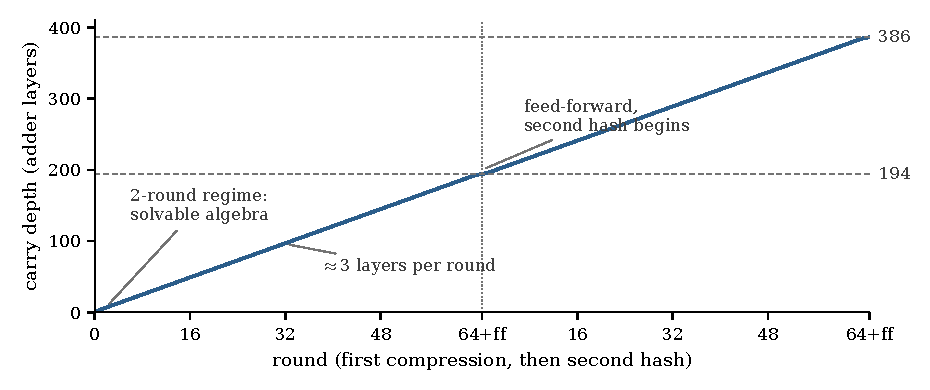
\includegraphics{figures/fig_depth_profile.pdf}
\caption{Carry depth along the SHA-256d dataflow, from the minimum-depth
accounting of \texttt{repro/carry\_depth.py}. The 64 rounds of the first
compression lift the state by roughly three adder layers per round, each
Davies--Meyer feed-forward adds a full-width carry layer, and the second
hash repeats the climb to $386$. The solvable two-round regime sits at
the origin.}
\label{fig:depth}
\end{figure}

\subsection{Measuring the per-layer retention: the anchor sweep}
\label{sec:anchor}

The depth fixes the exponent's base count ($386$); the margin is
$386\cdot\log_2(1/\rho)$, where $\rho$ is the advantage retained per
adder layer. We measure $\rho$ directly on real reduced $\SHA$ (see
\texttt{repro/anchor\_sweep.py}). The carry-aware score
$(T_1\!\gg\!24)+(T_2\!\gg\!24)$, read at an interior round, strongly
predicts that the top byte of $\mathtt{state}[0]$ is small one layer
downstream; we measure how that control decays as the observed target
moves deeper. Over $24$ message stems (header-prefix stand-ins; see the
code for the simplified setup) and $2^{22}$ candidates each
(standard error on the mean advantage $\approx 10^{-3}$):

\begin{center}
\begin{tabular}{lc}
\hline
depth from read point & retained advantage\\
\hline
$1$ adder layer (same round) & $0.8856 \pm 0.0005$\\
one round deeper ($\approx 3$ layers) & $\le 0.0011$ (consistent with $0$)\\
\hline
\end{tabular}
\end{center}

The advantage \emph{cliffs} (Figure~\ref{fig:cliff}): it falls from
$0.886$ to undetectable within a single round. There is no geometric tail to fit; $\rho \approx 0$
(a one-layer reset). The mechanism is explicit: at the next round
$\mathtt{state}[0]$ enters $\Sigma_0$, whose rotations scatter the
controlled top byte across all bit positions, and is then re-randomized
by a fresh carry chain, so the controlled structure is delocalized off
the top-byte observable in one round. Information is preserved (the round
is invertible); accessibility is destroyed.

\begin{figure}[t]
\centering
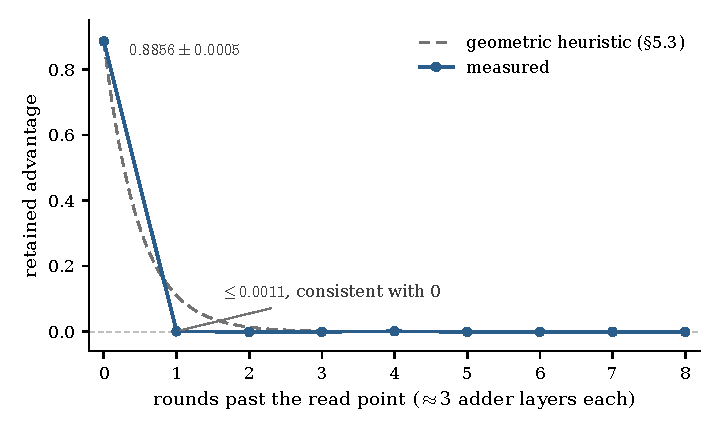
\includegraphics{figures/fig_anchor_cliff.pdf}
\caption{The anchor sweep (Section~\ref{sec:anchor}): selection advantage
of the carry-aware score read $j$ rounds past the read point, against the
geometric decay suggested by the carry Markov heuristic of
Section~\ref{sec:markov}. The measurement returns a cliff rather than a
slope; past one round every value sits within the $\approx 10^{-3}$
detection limit of zero.}
\label{fig:cliff}
\end{figure}

\subsection{The combined statement}

The target output sits $386$ adder layers from the controllable header
inputs, while the strongest local advantage we measured has reach of
about one layer and is dead within a single round ($\approx 3$ layers).
The margin therefore does not rest on a thin
$\rho^{386}$ extrapolation; the advantage is already gone roughly $100$
rounds before the output. We deliberately do not compound the measured
one-sided bound $\rho_{\text{round}}\le 0.0011$ (a $2\sigma$ upper bound
on the deeper-round mean advantage) across the remaining rounds: that
bound is a detection limit consistent with $\rho=0$, not a measured decay
rate, and multiplying it would manufacture a precise-looking exponent from
what is in fact a null result. The honest statement needs no
extrapolation---the advantage is already below detection after a single
round, and $\SHAd$ applies $128$ rounds.

\paragraph{Relation to circuit-complexity measures.}
Carry depth should not be conflated with the circuit measures it
superficially resembles. The closest prior notion is the carry-truncation
depth of Field and Jones~\cite{fieldjones}, who independently identify the
carry as the sole nonlinearity of ARX; their depth is a local
approximation parameter on a single addition, whereas carry depth is an
exact, global count of carry layers along the input-to-output dataflow of
the whole function. It is likewise distinct from the FHE/MPC notion of
\emph{multiplicative} (AND) \emph{depth}: the standard Bristol-Fashion
circuit for one $\SHA$ compression has AND-depth $1607$~\cite{bristol,multdepth},
far above our $386$, because AND-depth counts every nonlinear gate on the
path---including the bit-local $\Ch$/$\Maj$ gates and every gate of a
ripple-carry adder---while carry depth counts only carry layers and
assigns $\Ch$/$\Maj$ depth $0$. Crucially, AND-depth is a property of a
chosen circuit: the same modular addition has linear AND-depth as
ripple-carry but logarithmic depth as a parallel-prefix
adder~\cite{cla}, since the carry-merge operator is associative, and
published heuristics shrink a $128$-bit adder from AND-depth $255$ to $9$
without altering its logic~\cite{multdepth}. Carry depth, by contrast,
counts the logical carry-dependency layers and is invariant to the
realization---it is a coordinate of the function, not of an
implementation. Nor is it multiplicative \emph{complexity}, a gate
\emph{count} (an $n$-bit adder needs exactly $n{-}1$ AND
gates~\cite{boyarperalta}) carrying no notion of depth.

% =====================================================================
\section{Scope and the residual}\label{sec:scope}
% =====================================================================

Every statement in Section~\ref{sec:carry} is conditional on the attack
belonging to the \emph{carry / local-structure class}. This is the
natural class, since carries are the only position-coupling nonlinearity.
The carry-aware score we measured is a strong, natural member of it---a
single observable read by a single score at a single interior round---and
its reach is about one layer, dead within a single round; we do not claim
to have exhausted the class, and a broader sweep over observables, scores,
and read points is the obvious next test. The analysis does not bound a hypothetical local
attacker with longer reach; that possibility is the same residual isolated
by Theorem~\ref{thm:reduction}.

The residual is a single, well-defined object: \emph{a global algebraic
shortcut that resolves the target output without resolving the carries on
the path}. By the standard-model reduction, such a shortcut is a
distinguisher against $\SHA$, which is to say a cryptographic break. We
cannot prove it does not exist; as discussed in
Section~\ref{sec:search}, an unconditional exclusion would require
explicit circuit lower bounds beyond current techniques. The public
cryptanalytic record of $\SHA$ is the empirical statement that no such
shortcut has been found.

The honest ceiling is therefore that mining cannot beat brute force
unless $\SHA$ is broken. We have bounded the search unconditionally in
the ideal model, reduced the standard-model claim to a $\SHA$
distinguisher, explained why the natural attack class has no reach, and
quantified that the structural separation ($386$ layers) is far larger
than the measured reach ($\sim 1$ layer).

\paragraph{Empirical consistency.}
Independent of the theory, we ran the natural attack families against
$\SHAd$ targets and found no advantage, exactly as the theory predicts:
selection by any function of the first-hash digest's lexicographic order
(an oracle for the smallest first-hash digest produces no signal at the
$\SHAd$ output, because the second hash decorrelates input order from
output order); shallow round-internal carry, Boolean, and
message-schedule features under pre-registered, multiple-testing-corrected
tail-hit gates; and per-block-template stem selection under an
extreme-value yield model. To check that the cliff is not an artifact of a
weak hand-built score, we also trained a neural distinguisher in the style
of Gohr's attack on round-reduced ARX~\cite{gohr}: a residual network
given, as features, everything computed through the read round---the state
words, their carry-free derivations, the round's modular sums, and the
schedule words, in bit, value, and Fourier encodings---and free to learn
any function of them. Although it \emph{exceeds} the hand-built carry-aware
score one adder layer downstream ($0.998$ versus $0.88$ retained
advantage), its advantage collapses to the noise floor one round deeper,
across independent stems and at a shifted read point, and remains null
under a $90\times$ model-capacity, $64\times$ training-data, and $8\times$
training-time scaling of the learned attacker (each scaled run compared
against its own shuffled-label noise ceiling)---the same single-round
cliff, now traced by a strictly stronger member of the attack class
(Figure~\ref{fig:neural}a).
Control runs locate the failure at the mechanism itself: the same
architecture learns the top byte of pure $k$-operand modular sums for
$k\le3$ and fails for $k\ge4$ (Figure~\ref{fig:neural}b), so the learned
attacker expires on carry composition as such, on data with no $\SHA$
structure at all. This $k\ge4$ failure is a genuine
optimisation/trainability barrier, not an artefact of finite feature
precision: it survives rebuilding the operand features and the entire
network in double precision (a seed-paired \texttt{float32}-vs-\texttt{float64}
comparison leaves the advantage at the noise floor in both arms, $0/6$
seeds learning in either precision), so restoring full operand resolution
does not let gradient descent find the carry circuit. The same carry-depth mechanism that bounds the
attack class also \emph{retrodicts} the qualitative behaviour observed in
those experiments, in particular the round-invariance of the local
advantage (it is always a depth-one quantity) and its destruction by the
chaining-variable addition (a single extra carry layer).

\begin{figure}[t]
\centering
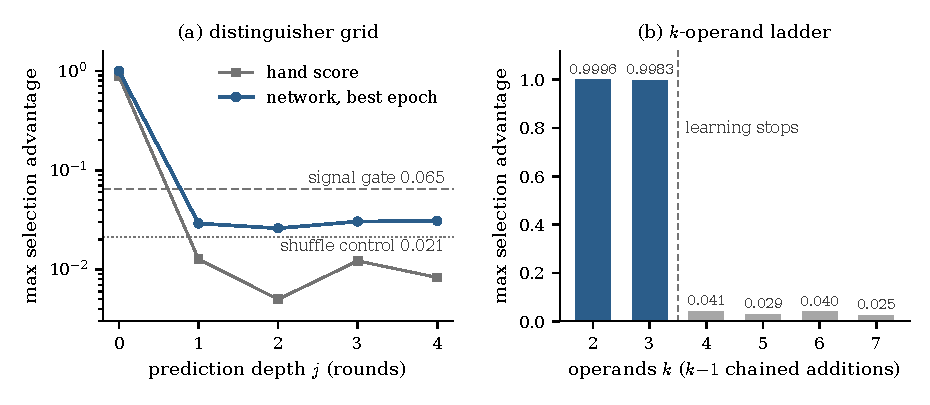
\includegraphics{figures/fig_neural.pdf}
\caption{The learned attacker. (a)~Maximum selection advantage of the
neural distinguisher and the hand-built score across prediction depths,
against the pre-registered candidate-signal gate and the shuffled-label
control: the network beats the hand score where signal exists ($j=0$)
and joins the noise floor one round deeper. (b)~The same architecture on
pure $k$-operand modular sums, no $\SHA$ structure present: two chained
additions are learnable, three are not.}
\label{fig:neural}
\end{figure}

% =====================================================================
\section{Reproduction}\label{sec:repro}
% =====================================================================

The two quantitative results are reproducible from self-contained code in
\texttt{repro/}, built on a vendored minimal $\SHA$ verified bit-exact
against \texttt{hashlib}:
\begin{itemize}
\item \texttt{carry\_depth.py}, the exact $386$-layer dataflow
  accounting (pure Python, no dependencies, instant);
\item \texttt{anchor\_sweep.py}, the per-layer advantage measurement
  ($0.886$ at depth one, consistent with $0$ one round deeper); the full
  run uses \texttt{numpy}/\texttt{cupy}, and a \texttt{-{}-pure}
  standard-library-only smoke path reproduces the cliff (and a
  \texttt{hashlib} parity check) in seconds on any interpreter;
\item \texttt{sha256\_ref.py}, the vendored $\SHA$ and its parity
  check.
\end{itemize}
The neural-distinguisher experiment of Section~\ref{sec:scope} is
likewise reproducible, from \texttt{neural/}
(pre-registered protocol with documented amendments, training code, and
raw per-cell results); unlike the two results above it requires a GPU
and the JAX/optax stack.

% =====================================================================
\section{Related work and conclusion}\label{sec:related}
% =====================================================================

Proof-of-work security is conventionally proved in the random-oracle
model~\cite{backbone}, with standard-model~\cite{gkp} and
post-quantum~\cite{pqbackbone,hybrid} analyses extending it. As we make
explicit, the impossibility of beating brute force is not provable
unconditionally in the standard model without resolving open hardness
questions. ASICBoost~\cite{asicboost} is the canonical input-side win,
and it occupies the only shareable region we identify. The role of
modular addition as the nonlinear primitive of ARX constructions is well
studied~\cite{arx,sfunction}, and the carry as its sole nonlinearity has
been observed before~\cite{fieldjones}; our contribution is to turn this
into \emph{carry depth}, an explicit, circuit-independent coordinate of
the proof-of-work function space, to compute it exactly for $\SHAd$, and
to measure that the strongest local advantage has reach of about one
layer (dead within a single round), so
that the $386$-layer separation is decisive rather than marginal.
Auxiliary-input bounds~\cite{cdgs,cdg,unruh,dgk} and the BBBV quantum
lower bound~\cite{bbbv} close the preprocessing and quantum loopholes. The
public cryptanalytic record is consistent with this ceiling: reduced-round
collision attacks reach only $31$ of $64$ steps (made practical
in~\cite{lll24}, building on~\cite{mendel13}) and $39$ steps
semi-free-start~\cite{lll24}, and preimages reach $43$ steps at cost
$2^{254.9}$~\cite{aoki09}, all far from the full function.

SHA-256d mining cannot beat brute force by any route we or the
cryptanalytic record can find, and cannot at all unless $\SHA$ is broken.
The only standing economic wins are the known constant-factor sharing
techniques, and they are bounded.

% =====================================================================
\begin{thebibliography}{99}

\bibitem{backbone}
J.~Garay, A.~Kiayias, N.~Leonardos.
\emph{The Bitcoin Backbone Protocol: Analysis and Applications.}
EUROCRYPT 2015.

\bibitem{asicboost}
T.~Hanke.
\emph{AsicBoost: A Speedup for Bitcoin Mining.}
2016, \texttt{arXiv:1604.00575}.

\bibitem{unruh}
D.~Unruh.
\emph{Random Oracles and Auxiliary Input.}
CRYPTO 2007.

\bibitem{cdgs}
S.~Coretti, Y.~Dodis, S.~Guo, J.~Steinberger.
\emph{Random Oracles and Non-Uniformity.}
EUROCRYPT 2018.

\bibitem{cdg}
S.~Coretti, Y.~Dodis, S.~Guo.
\emph{Non-Uniform Bounds in the Random-Permutation, Ideal-Cipher, and
Generic-Group Models.}
CRYPTO 2018.

\bibitem{bbbv}
C.~Bennett, E.~Bernstein, G.~Brassard, U.~Vazirani.
\emph{Strengths and Weaknesses of Quantum Computing.}
SIAM J.\ Comput.\ 26(5), 1997.

\bibitem{arx}
H.~Lipmaa, S.~Moriai.
\emph{Efficient Algorithms for Computing Differential Properties of
Addition.}
FSE 2001.

\bibitem{coron}
J.-S.~Coron, Y.~Dodis, C.~Malinaud, P.~Puniya.
\emph{Merkle-Damg\aa rd Revisited: How to Construct a Hash Function.}
CRYPTO 2005.

\bibitem{drst}
Y.~Dodis, T.~Ristenpart, J.~Steinberger, S.~Tessaro.
\emph{To Hash or Not to Hash Again? (In)differentiability Results for
$H^2$ and HMAC.}
CRYPTO 2012.

\bibitem{gkp}
J.~Garay, A.~Kiayias, G.~Panagiotakos.
\emph{Proofs of Work for Blockchain Protocols.}
IACR Cryptology ePrint Archive, Report 2017/775, 2017.

\bibitem{pqbackbone}
A.~Cojocaru, J.~Garay, A.~Kiayias, F.~Song, P.~Wallden.
\emph{Quantum Multi-Solution Bernoulli Search with Applications to
Bitcoin's Post-Quantum Security.}
Quantum 7:944, 2023.

\bibitem{hybrid}
A.~Cojocaru, J.~Garay, F.~Song.
\emph{Generalized Hybrid Search with Applications to Blockchains and Hash
Function Security.}
ASIACRYPT 2024.

\bibitem{dgk}
Y.~Dodis, S.~Guo, J.~Katz.
\emph{Fixing Cracks in the Concrete: Random Oracles with Auxiliary Input,
Revisited.}
EUROCRYPT 2017.

\bibitem{hellman}
M.~E.~Hellman.
\emph{A Cryptanalytic Time-Memory Trade-Off.}
IEEE Trans.\ Inf.\ Theory 26(4), 1980.

\bibitem{rainbow}
P.~Oechslin.
\emph{Making a Faster Cryptanalytic Time-Memory Trade-Off.}
CRYPTO 2003.

\bibitem{mrh}
U.~Maurer, R.~Renner, C.~Holenstein.
\emph{Indifferentiability, Impossibility Results on Reductions, and
Applications to the Random Oracle Methodology.}
TCC 2004.

\bibitem{rss}
T.~Ristenpart, H.~Shacham, T.~Shrimpton.
\emph{Careful with Composition: Limitations of the Indifferentiability
Framework.}
EUROCRYPT 2011.

\bibitem{sfunction}
N.~Mouha, V.~Velichkov, C.~De Canni\`ere, B.~Preneel.
\emph{The Differential Analysis of S-functions.}
SAC 2010.

\bibitem{fieldjones}
R.~E.~Field, B.~C.~Jones.
\emph{Using Carry-Truncated Addition to Analyze Add-Rotate-Xor Hash
Algorithms.}
2013, \texttt{arXiv:1303.4448}.

\bibitem{boyarperalta}
J.~Boyar, R.~Peralta.
\emph{Tight Bounds for the Multiplicative Complexity of Symmetric
Functions.}
Theoretical Computer Science 396, 2008.

\bibitem{multdepth}
P.~Aubry, S.~Carpov, R.~Sirdey.
\emph{Faster Homomorphic Encryption is not Enough: Improved Heuristic for
Multiplicative Depth Minimization of Boolean Circuits.}
CT-RSA 2020.

\bibitem{bristol}
N.~P.~Smart et al.
\emph{`Bristol Fashion' MPC Circuits.}
\texttt{https://nigelsmart.github.io/MPC-Circuits/}.

\bibitem{cla}
T.~G.~Draper, S.~A.~Kutin, E.~M.~Rains, K.~M.~Svore.
\emph{A Logarithmic-Depth Quantum Carry-Lookahead Adder.}
Quantum Inf.\ Comput.\ 6(4), 2006.

\bibitem{lll24}
Y.~Li, F.~Liu, G.~Wang.
\emph{New Records in Collision Attacks on SHA-2.}
EUROCRYPT 2024.

\bibitem{mendel13}
F.~Mendel, T.~Nad, M.~Schl\"affer.
\emph{Improving Local Collisions: New Attacks on Reduced SHA-256.}
EUROCRYPT 2013.

\bibitem{aoki09}
K.~Aoki, J.~Guo, K.~Matusiewicz, Y.~Sasaki, L.~Wang.
\emph{Preimages for Step-Reduced SHA-2.}
ASIACRYPT 2009.

\bibitem{bip320}
\emph{nVersion Bits for General Purpose Use (BIP~320).}
Bitcoin Improvement Proposals, 2018.

\bibitem{gohr}
A.~Gohr.
\emph{Improving Attacks on Round-Reduced Speck32/64 Using Deep Learning.}
CRYPTO 2019.

\end{thebibliography}

\end{document}
